%---------------- COMMENT FOR IMPORTING ----------------------
%\RequirePackage{lineno}				
%\documentclass[12pt]{report}		
%\pagestyle{headings}
%\input{ST-input2}							

%\setcounter{chapter}{0}
%\begin{document}								
%\setpagewiselinenumbers
%\linenumbers
%\tableofcontents
\graphicspath{{Appendix/figures_B/}} 
%-------------------------------------------------------------

\chapter{Supplementary Material on Compressive Sensing}
\label{chap:ap_B}

The purpose of this appendix is to provide supplementary material on compressive sensing. An introduction to compressive sensing is given in Section \ref{sec:intro_cs}. The conditions for choosing a stable measurement matrix $\boldsymbol{\Phi}$ are described in Section \ref{sec:sensing-matrices} and more intuition is provided on the orthogonal matching pursuit algorithm  in Section \ref{sec:intuition_omp}.




% Often, signals may not appear to be compressible until a transformation is applied to them, a classic example of this comes from the subject of image processing. It is well known that natural images can be well represented by using wavelets \cite{mallat1999wavelet}. Figure \ref{fig:waveletcoeff} depicts a natural image and its corresponding  wavelet transform. The original image in its raw form is not directly suitable for compressed sensing, but after the wavelet transformation the signal is in a compressible form. The lighter pixels in Figure \ref{fig:wt} represent large coefficients from the wavelet transform and dark pixels represent small coefficients, so light areas determine where most of the information in the image is stored. There are many areas of dark in Figure \ref{fig:wt} but only a few light areas, meaning that the image is compressible, although that was not obvious from Figure \ref{fig:ri} alone.

% \begin{figure}[h]
%   \centering
%    \begin{subfigure}[b]{0.4\textwidth}
%                 \centering
%                 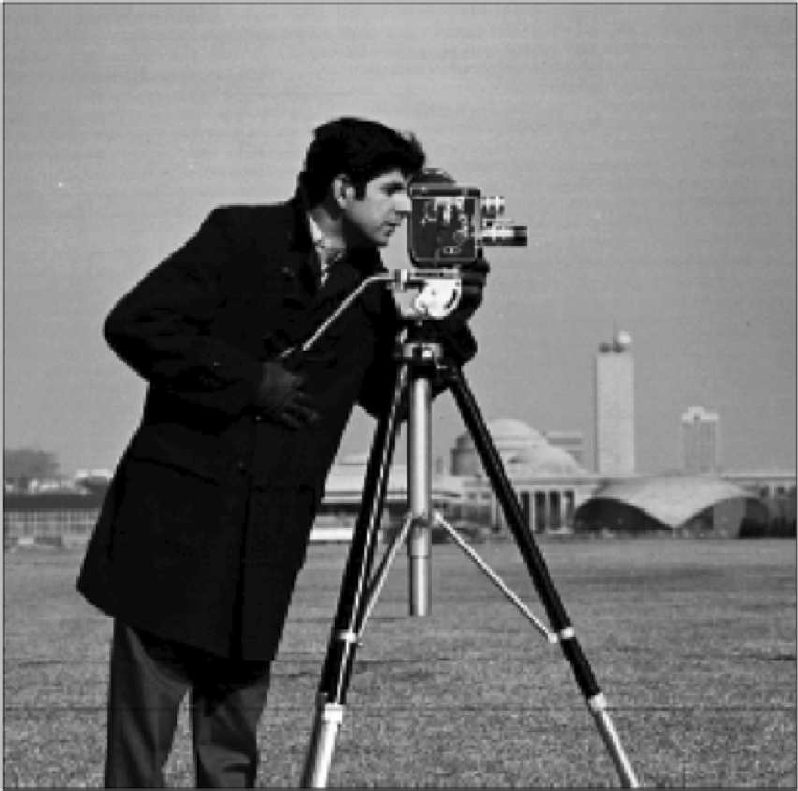
\includegraphics[width=\textwidth]{manoriginal}
%                 \caption{Original frame}
% \label{fig:ri}
%         \end{subfigure}
% \quad
% \begin{subfigure}[b]{0.4\textwidth}
%                 \centering
%                 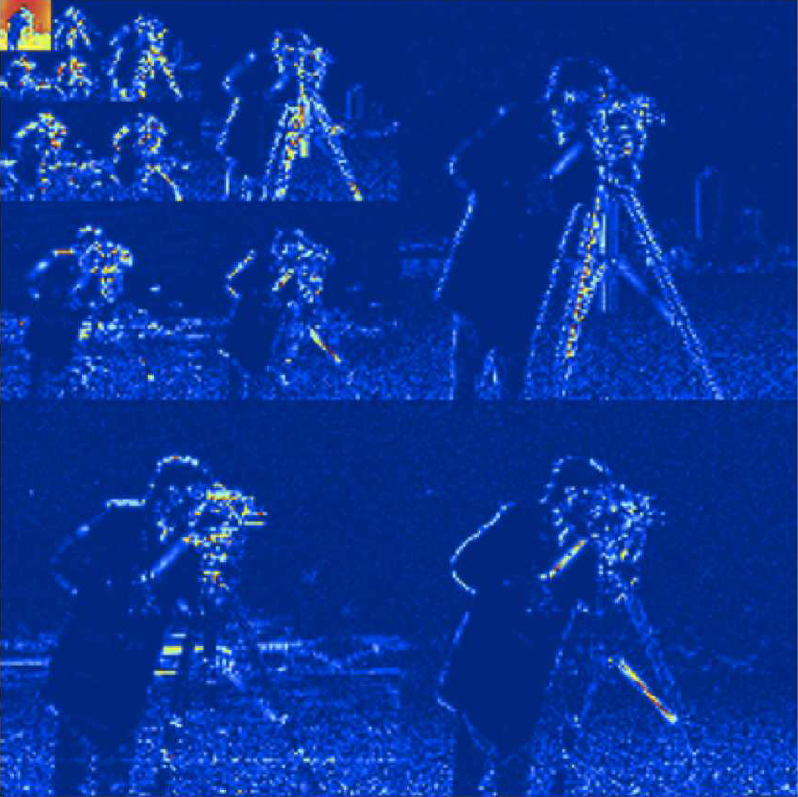
\includegraphics[width=\textwidth]{manwavelet}
%                 \caption{Wavelet transformation}
%                 \label{fig:wt}
%         \end{subfigure}
%   \caption{A natural image and its wavelet transform. In the wavelet transformation lighter pixels refer to large transform coefficients and dark areas refer to smaller coefficients. There are only few light areas but many dark ones which implies that the image is compressible. Figure originally appears in \cite{Baraniuk2011}.}
%   \label{fig:waveletcoeff}
% \end{figure}

%Many signals are sparse in their construction, or can be manipulated into a sparse or compressible form by applying sparsity transforms such as the wavelet decomposition for natural images. The simplistic, compact form of these signals make them ideal for many areas, particularly when storage and computational power is important. The work of compressive sensing provides a framework to randomly sample and later recover compressible signals well.

\section{Introduction to Compressive Sensing}
\label{sec:intro_cs}



Compressive sensing \citep{Candes2006, Candes2006a, Donoho2006} is  based on the discovery that there is a way to accurately sample a signal at a much lower frequency than the Nyquist frequency, provided that the signal that you are trying to sample is either sparse or compressible.
The definition of a sparse signal is given below.
%Sparsity can be a very desirable condition for signals to exhibit, as the presence of sparsity can reveal hidden structures and provide a compact and therefore simple representation of the signals.  If many ways to represent a signal exist, then seeking a sparse representation can often be the best option.



\begin{mydef}
  A signal $\boldsymbol{x} \in \mathbb{R}^{N}$ is known as being $K$-sparse if it can be represented as a linear combination of $K$ basis vectors.  
 \end{mydef}

In simpler terms, we can think of a signal being $K$-sparse if it can transformed so that it contains at most $K$ non-zero elements, or written mathematically,  

 \begin{equation*}
    \label{eq:100}
\|\boldsymbol{x}\|_{0} \leq K .   
  \end{equation*}

For notational purposes, we express the set of all $K$-sparse signals as 

\begin{equation*}
  \label{eq:21}
  \Sigma_{K} = \{\boldsymbol{x}:\|\boldsymbol{x}\|_{0} \leq K\}. 
\end{equation*}

Generally the signal of interest is not exactly sparse but approximately sparse, which is also known as compressible. For a signal to be compressible we still require $K$ large coefficients (with $K << N$) but the remaining $N-K$ coefficients are only required to be small and not necessarily zero.

% A compressible signal can be well-approximated but not necessarily exactly replicated by its sparse representation.  Fundamentally a signal is compressible if most of the information in the signal is represented by a few coefficients. 



The compressive sensing theory describes how a finite compressible signal $\boldsymbol{x} \in \mathbb{R}^N$ can be recovered from a set of $M$ linear, non-adaptive measurements $\boldsymbol{y}$ where $M < < N$. The measurement $\boldsymbol{y}$ is a linear function of the signal $\boldsymbol{x}$ as shown in equation \eqref{eq:10_Ap} or visualised in Figure \ref{fig:csVC}. The number of measurements $M$ in $\boldsymbol{y}$ is assumed to be smaller than signal $\boldsymbol{x}$, so we choose a measurement matrix $\boldsymbol{\Phi} \in R^{M \times N}$ with $M < < N$. It is known from linear algebra that there are infinitely many vectors $\boldsymbol{x}$ that can solve equation \eqref{eq:10_Ap}, but usually $\boldsymbol{x}$ is the only sparse solution, provided that $M \geq 2K$, where $K$ is the true sparsity of the signal. Therefore if $\boldsymbol{x}$ is known in advance to be sparse, it can in theory be reconstructed exactly from $M$ measurements.
%
\begin{equation}
  \label{eq:10_Ap}
\boldsymbol{y} =\boldsymbol{\Phi x}.
\end{equation}
%


\begin{figure}[h]
  \centering
  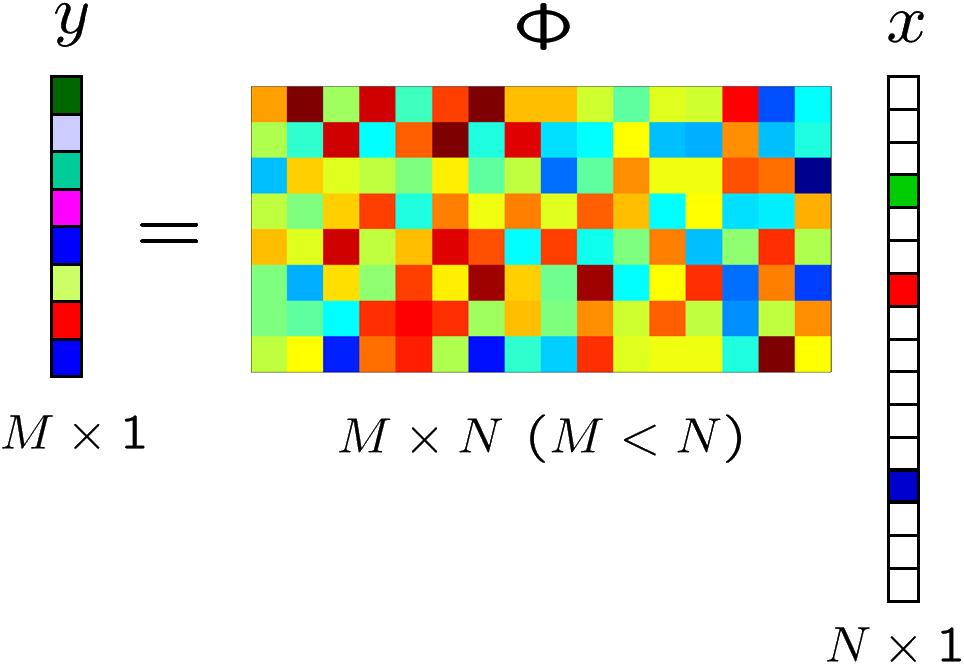
\includegraphics[width = 9cm]{csss.png}
\caption{A visualisation of the signal acquirement process in compressive sensing. A sparse signal $\boldsymbol{x}$ of length $N$ is under sampled by multiplication of a random measurement matrix $\boldsymbol{\Phi}$, resulting in the non-sparse measurement vector $\boldsymbol{y}$ of much smaller length $M$. Courtesy of Volkan Cevher.}
\label{fig:csVC}
\end{figure}

Compressive sensing is different from classical sampling in a number of ways. The two main differences are the manner in which measurements are acquired, and how the signal is reconstructed from these measurements.

%, named after Claude Shannon and Harry Nyquist,
 In classical sampling, measurements are taken at equidistant intervals at a frequency above the Nyquist frequency. The Shannon-Nyquist theorem \citep{Shannon1949} allows analogue signals to be digitally sampled and later restored back to an analogue signal accurately. In order for the signal to be reconstructed uniquely from its digital sample, it must be sampled at a rate  above the Nyquist Sampling frequency. This frequency is defined to be twice the bandwidth of the signal, where the bandwidth refers to the highest frequency present in the signal.  In contrast, in compressive sensing sampling occurs at randomly spaced intervals in accordance with a measurement matrix $\boldsymbol{\Phi}$, the choice of which is discussed in Section \ref{sec:sensing-matrices}. 

The method of signal reconstruction also differs between classical and compressive sensing. If the signal has been sampled in accordance with the Shannon-Nyquist theorem, the Whittaker-Shannon interpolation formula is applied in order to reconstruct the signal accurately. However, when dealing with compressed signals things are not so simple. We need to be able to determine the significant coefficients of some sparse representation of the signal and calculate a least squares approximation. This is not straightforward to calculate exactly in practise and instead a recovery algorithm is used to get an optimal solution. In Section \ref{sec:intuition_omp} we introduce one such recovery algorithm and provide intuition on how it is able to recover sparse signals. %%%%%The choice of this recovery algorithm will be discussed further in Section \ref{sec:recovery-algorithms}.

% \begin{example}
%   \label{sec:sparse-compr-sign}
%   Let $\boldsymbol{x}$ be a discrete signal of length 256, which is directly 20-sparse therefore exactly 20 of its elements are non-zero. The signal can be represented as in Figure \ref{fig:ex1}. How many samples are required to capture this signal efficiently? As the signal isn't bandlimitted, according to the Shannon Nyquist theorem we would need to sample all 256 elements in order to reconstruct the signal correctly. However if the logic of compressive sensing is applied, it is possible to sample using fewer than 256 measurements, because the signal exhibits the sparsity property. Lets take $M = 100$ measurements by creating a measurement matrix $\boldsymbol{\Phi}$ and multiplying it by the signal $\boldsymbol{x}$ as shown in equation \eqref{eq:10}. Assuming that the measurement matrix is well defined (Section \ref{sec:sensing-matrices}) it is possible to recover the signal $\boldsymbol{x}$ from only the information stored in $\boldsymbol{y}$. In order to estimate $\boldsymbol{y}$, a recovery algorithm (Section \ref{sec:recovery-algorithms}) is applied to $\boldsymbol{y}$ and the result is shown in Figure \ref{fig:exDONE}. The signal has been recovered perfectly using less than $40\%$ of the available measurements. 

% \begin{figure}
%         \centering
%         \begin{subfigure}[b]{0.5\textwidth}
%                 \centering
%                 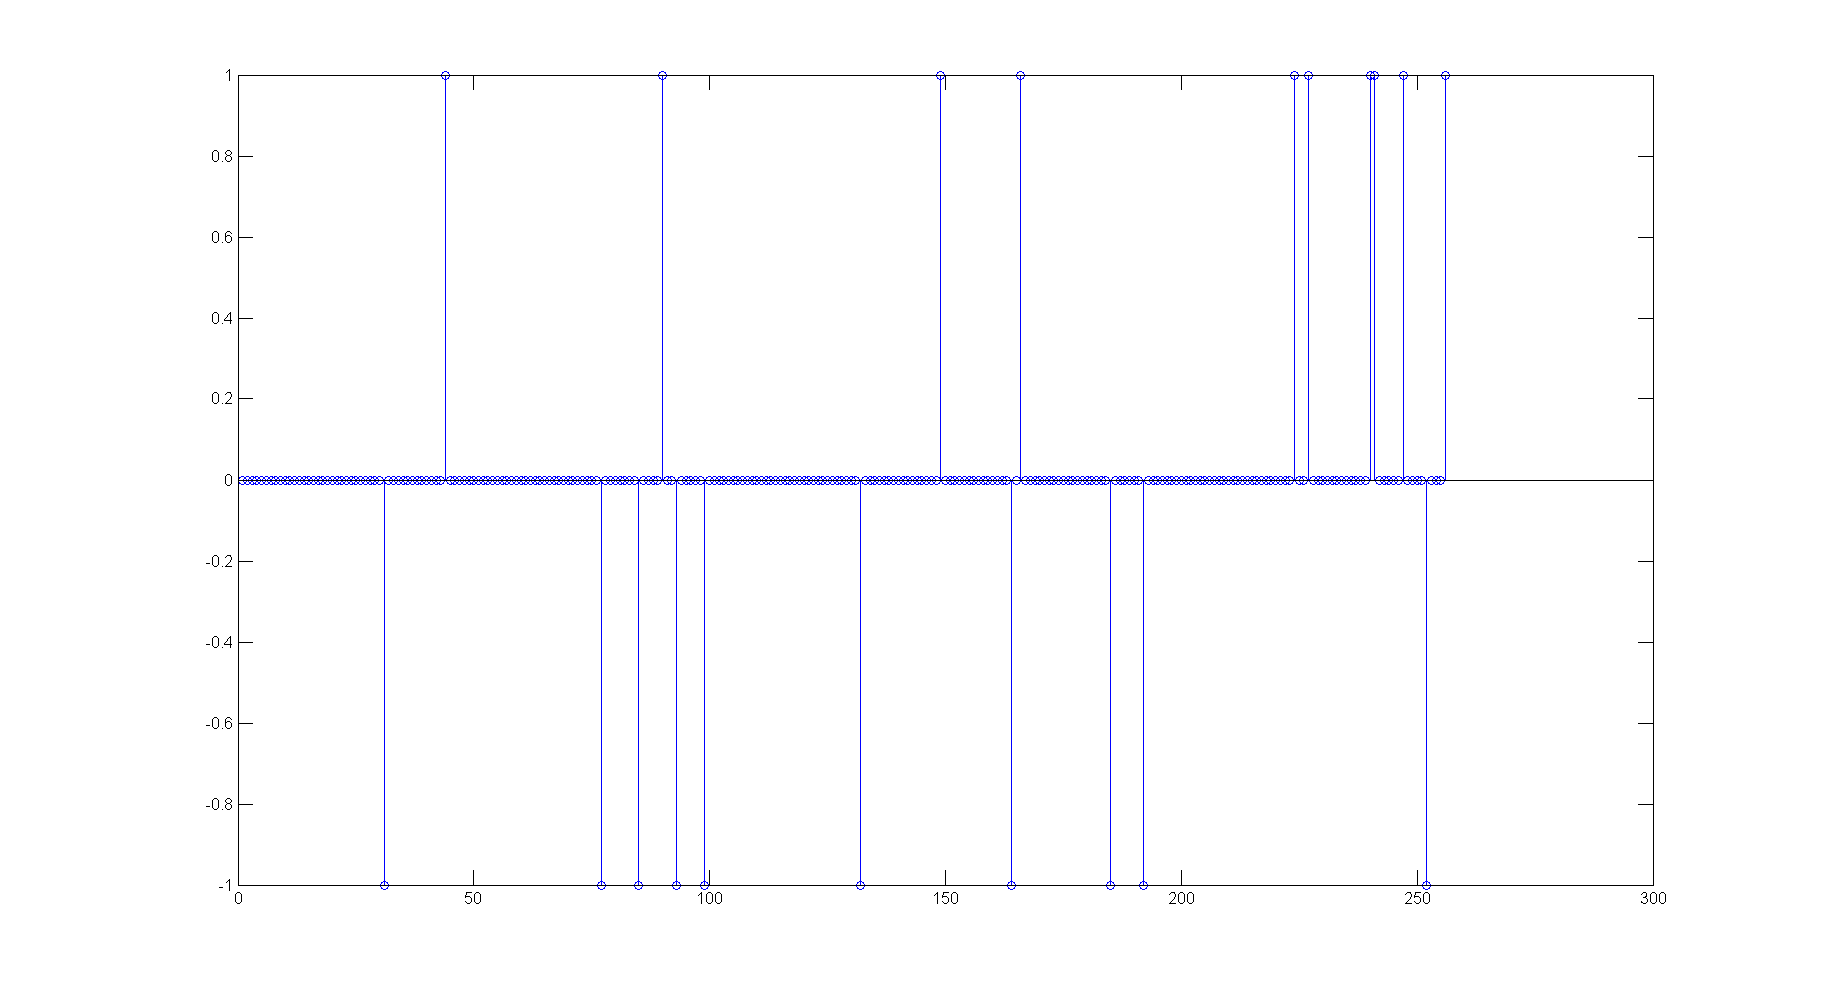
\includegraphics[width=\textwidth]{ex1}
%                 \caption{The original signal $\boldsymbol{x}$}
%                 \label{fig:ex1}
%         \end{subfigure}%
%         ~ %add desired spacing between images, e. g. ~, \quad, \qquad etc.
%           %(or a blank line to force the subfigure onto a new line)
%         \begin{subfigure}[b]{0.5\textwidth}
%                 \centering
%                 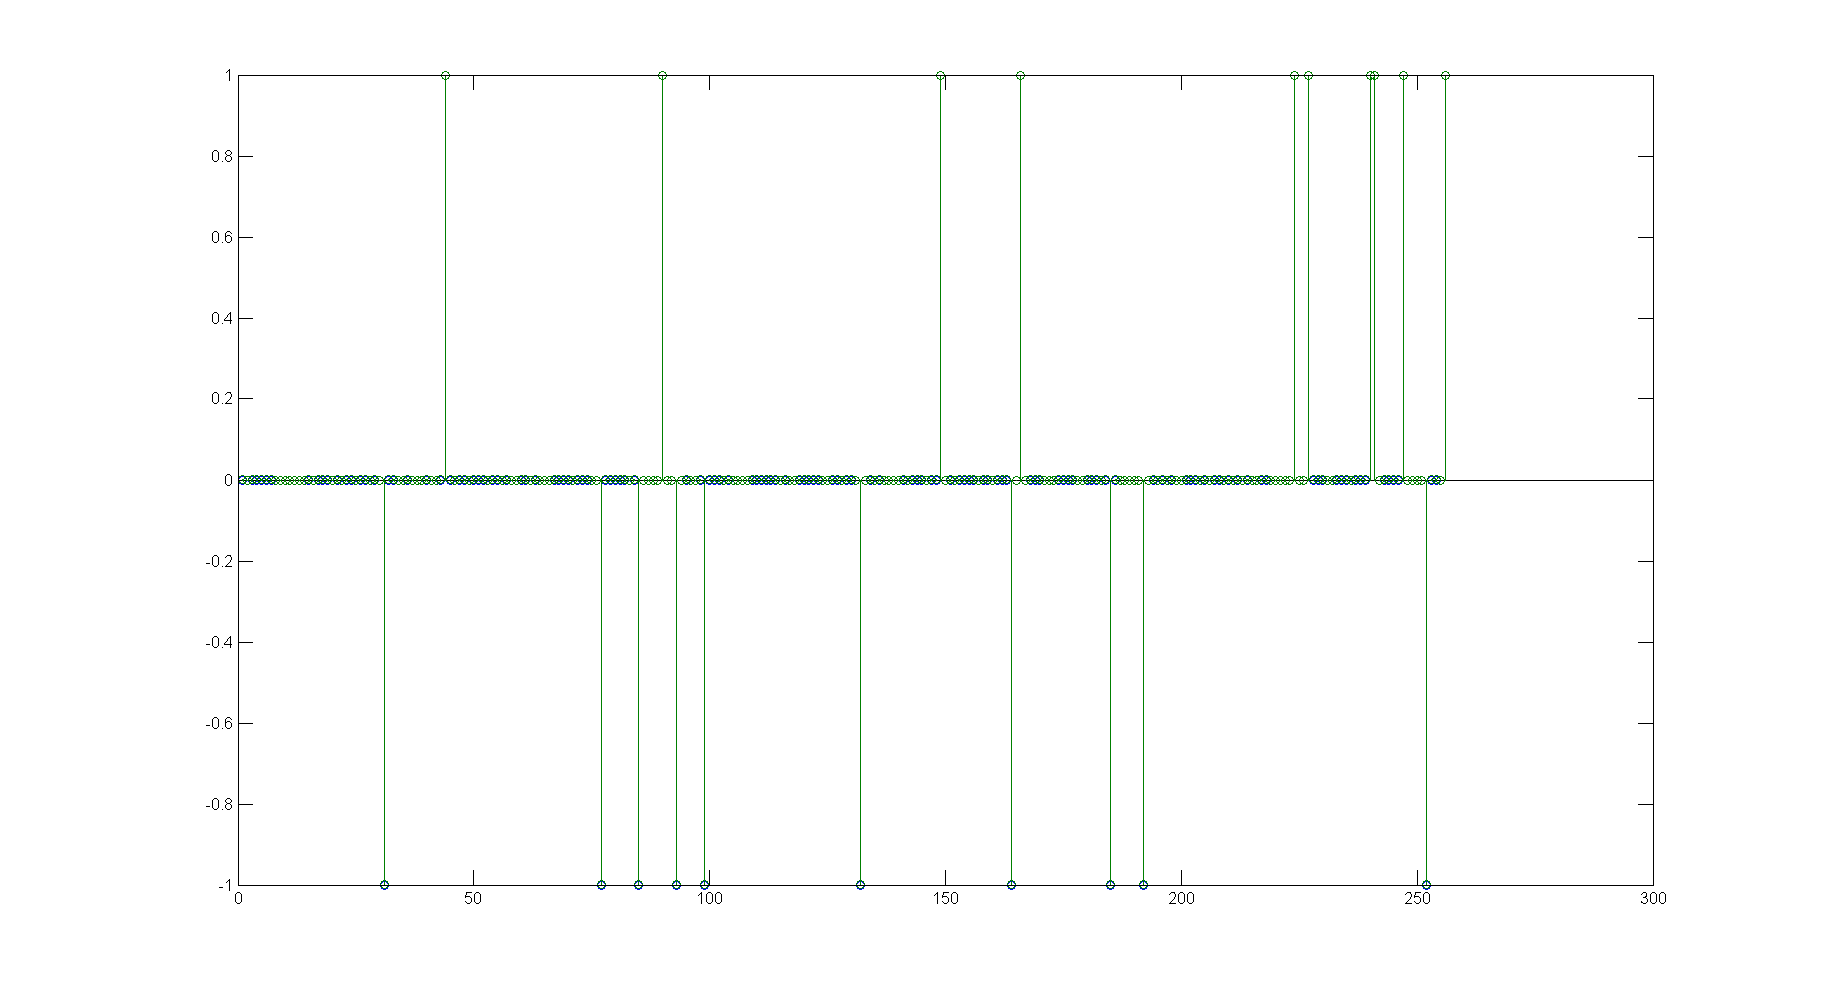
\includegraphics[width=\textwidth]{exDONE}
%                 \caption{The recovered signal $\boldsymbol{\hat{x}}$}
%                 \label{fig:exDONE}
%         \end{subfigure}
% %\caption{ }\label{fig:sparse}
% \end{figure}


% \end{example}


%Now that compressive sensing has been introduced, the specifics of choosing a suitable sensing matrix and recovery algorithm are discussed in Sections \ref{sec:sensing-matrices} and \ref{sec:recovery-algorithms} respectively.




\section{Conditions for a Stable Measurement Matrix}
\label{sec:sensing-matrices}
The matrix $\boldsymbol{\Phi}$ represents a dimensionality reduction as it maps the signal from $\mathbb{R}^N$ to $\mathbb{R}^M$.  It is of vital importance that we are able to design a stable measurement matrix $\boldsymbol{\Phi}$ so that the signal information is not damaged by the dimensional reduction from $\boldsymbol{x} \in \mathbb{R}^N$ to $\boldsymbol{y} \in \mathbb{R}^M$. In order to guarantee this, a number of conditions must be true for the measurement matrix $\boldsymbol{\Phi}$.

\subsection{Null Space Conditions}
\label{sec:null-space-property}

The first important property that is required is that the signal $\boldsymbol{x}$ can be uniquely reconstructed. It is possible to show that this will hold true if the null space $\mathcal{N}(\boldsymbol{\Phi})$ does not contain any vectors in $\Sigma_{2K}$. The Null space of $\boldsymbol{\Phi}$ is defined as follows,

\begin{equation}
  \mathcal{N}(\boldsymbol{\Phi}) = (\boldsymbol{z}:\boldsymbol{\Phi}\boldsymbol{z}=0). 
\end{equation}

In order to preserve $\boldsymbol{x} \in \Sigma_K$, it is required $\boldsymbol{\Phi x} \neq \boldsymbol{\Phi x^{\prime}} \; \forall  \boldsymbol{x^{\prime}} \in \Sigma_K$, because  if $\boldsymbol{\Phi x} = \boldsymbol{\Phi x^{\prime}}$ it would be impossible to distinguish $\boldsymbol{x}$ from $\boldsymbol{x^{\prime}}$ based only on $\boldsymbol{y}$. Consider the case where $\boldsymbol{\Phi x} = \boldsymbol{\Phi x^{\prime}}$.
\begin{align*}
  \boldsymbol{\Phi x} &= \boldsymbol{\Phi x^{\prime}} \\
& \Rightarrow \boldsymbol{\Phi}(\boldsymbol{x} - \boldsymbol{x^{\prime}}) = 0\\
&\Rightarrow (\boldsymbol{x} - \boldsymbol{x^{\prime}}) \in \Sigma_{2K}.
\end{align*}

This leads us to the conclusion that $\boldsymbol{\Phi}$ uniquely represents all $\boldsymbol{x} \in \Sigma_K \iff v \notin \mathcal{N}( \boldsymbol{\Phi}) \; \forall \boldsymbol{v} \in \Sigma_{2K}$. 
It can be shown that a bound on the spark of $\boldsymbol{\Phi}$ can characterise this property well. The spark of a matrix is defined in equation \eqref{eq:989} as the smallest number of columns of the matrix that are linearly dependent.

\begin{equation}
  \text{Spark}(\boldsymbol{\Phi}) = \min_{a \neq 0} \|a\|_0 : \boldsymbol{\Phi} a = 0. 
\label{eq:989}
\end{equation}

The spark can then be used to give the following guarantee as presented in \cite{eldar2012compressed}.

\begin{theorem}
  $\forall \boldsymbol{y}  \in \mathbb{R}^M \; \exists \; \text{ at most one } \boldsymbol{x} \in \Sigma_{K} : \boldsymbol{y} = \boldsymbol{\Phi}\boldsymbol{x} \; \iff \; \text{spark }(\boldsymbol{\Phi}) > 2K$.
\end{theorem}

\begin{proof}
  \label{sec:forall-boldsymb-in}
  Assume $\forall \boldsymbol{y} \in \mathbb{R}^M, \exists \text{ at most one signal } \boldsymbol{x} \in \Sigma_{K} : \boldsymbol{y} = \boldsymbol{\Phi}\boldsymbol{x}$. Assume $\text{spark }(\boldsymbol{\Phi}) \leq 2K$.  Due to the bound on the spark of $\boldsymbol{\Phi}$, there exists a set of at most $2K$ columns that are linearly dependent which implies that there exists some $\boldsymbol{v} \; \in \mathcal{N}(\boldsymbol{\Phi}) : \boldsymbol{v} \in \Sigma_{2K}.$  It is possible to express $\boldsymbol{v} = \boldsymbol{x} - \boldsymbol{x^{\prime}}$ where $\boldsymbol{x}, \boldsymbol{x^{\prime}} \in \Sigma_{K}$. Since $\boldsymbol{v} \in \mathcal{N}(\boldsymbol{\Phi}),  \boldsymbol{\Phi}(\boldsymbol{x} - \boldsymbol{x^{\prime}}) = 0$, this implies that  $\boldsymbol{\Phi x} = \boldsymbol{\Phi x^{\prime}}.$ This is a contradiction of the assumption that there is at most one signal $\boldsymbol{x} \in \Sigma_{K}$ such that $\boldsymbol{y} = \boldsymbol{\Phi}\boldsymbol{x}$. Therefore consider $\text{spark }(\boldsymbol{\Phi}) > 2K$. 

Assume that there exists $\boldsymbol{x}, \boldsymbol{x^{\prime}} \in \Sigma_{K}$ such that $\boldsymbol{\Phi x} = \boldsymbol{\Phi x^{\prime}} = \boldsymbol{y}.$ Therefore it can be seen that $\boldsymbol{\Phi}(\boldsymbol{x} - \boldsymbol{x^{\prime}}) = 0$. By letting $\boldsymbol{v} =  \boldsymbol{x} - \boldsymbol{x^{\prime}}$ it is possible to write $\boldsymbol{\Phi}\boldsymbol{v} = 0$. But as the $\text{spark }(\boldsymbol{\Phi}) > 2K$ this implies that $ \boldsymbol{v} = 0 \Rightarrow \boldsymbol{x} =  \boldsymbol{x^{\prime}}$ as expected.
\end{proof}

Since $\text{Spark}(\boldsymbol{\Phi}) \in [2,M+1]$, in order to preserve $\boldsymbol{x}$ in the dimensionality reduction, we require $M > 2K$. 
 
\subsection{The Restricted Isometry Property}
\label{sec:restr-isom-prop}
Although null space conditions can accommodate for the uniqueness of reconstruction, they do not account for noise. It is possible that the measurement vector $\boldsymbol{y}$ may be corrupted by noise during the measurement process. In order for the reconstruction problem to be well-conditioned, it is necessary that ${\boldsymbol{\Phi}}$ holds the Restricted Isometry Property (RIP) \cite{Donoho2006} of order $2K$. 
\begin{mydef}
 A matrix $\boldsymbol{\Phi}$ satisfies the (RIP) of order $K$ if there exists a $\delta_K  \in (0,1)$ such that 
\begin{equation*}
  \label{eq:40}
  (1 - \delta_k)||\boldsymbol{x}||^2_2 \leq||\boldsymbol{\Phi} \boldsymbol{x}||^2_2 \leq (1 + \delta_k)||\boldsymbol{x}||^2_2,
\end{equation*}

for all $\boldsymbol{x} \in \sum_K = {\boldsymbol{x}:||\boldsymbol{x}||_0 \leq K} $. 
\end{mydef}

%WRONG?
%The $l_2$ norm is defined  in equation \eqref{eq:573}. 
%
%\begin{equation}
%\label{eq:573}
%  ||\boldsymbol{x}||_2 = \sum_{i=1}^{N}||\boldsymbol{x_i}^2||
%\end{equation}

If $\boldsymbol{\Phi}$ satisfies the RIP with order $2K$, then $\boldsymbol{\Phi}$ preserves the distance between any pair of $K$-sparse vectors. It is the preservation of distance which will give a stronger guarantee of robustness against noise. 

%Another essential condition when selecting a $\Phi$ is incoherence, which requires that the rows of $\boldsymbol{\Phi}$ cannot sparsely represent the columns of $\boldsymbol{\Psi}$, and vice versa the the rows of $\boldsymbol{\Psi}$ cannot sparsely represent the columns of $\boldsymbol{\Phi}$, which will ensure that $\boldsymbol{\hat{x}}$ is a unique solution.

Unfortunately the task of checking that a matrix satisfies the RIP and null space conditions is an NP-hard problem, but fortunately both of these conditions will hold true with high probability if $\boldsymbol{\Phi}$ is selected as a random matrix \citep{Baraniuk2007}. In order to construct $\boldsymbol{\Phi}$ as such, the elements  $\phi_{i,j}$  are chosen as independent realisations of some probability distribution. In Chapter \ref{chap:CSBGS}, $\phi_{i,j}$ are independent and identically distributed (i.i.d.) Gaussian random variables with mean 0 and variance  $\frac{1}{N}$, but other distributions can be used.

%Now that conditions  on the measurement matrix have been established to preserve $\boldsymbol{x}$, the signal reconstruction is considered.


%\section{Recovery Algorithms}
%\label{sec:recovery-algorithms}

% Right at the heart of compressive sensing theory is the ability for recovery algorithms to provide accurate signal estimations in an efficient manner. Recovery algorithms generally fall into two categories, those based on convex optimisation and greedy algorithms. One type of each algorithm is considered.

% \subsection{Convex Optimisation}
% \label{sec:convex-optimization}

% Convex optimisation is a minimisation problem subject to a number of constraints where the functions involved are convex. No general solver is applied to these problems, but many methods exist that can be applied. As seen in equation \eqref{eq:10} the encoding system is under determined, therefore there exist many possible solutions from which a best estimate needs to be selected. In addition, it is known that before encoding, the signal $\boldsymbol{x}$ was sparse in some form, which is the key factor which enables the decoding process.



% % in this problem we have an undetermined system, and so there exists many possible solutions, and we need to pick the most suitable solution, or the best estimate for our decoded signal. In addition we also have the knowledge that before encoding, the signal $\boldsymbol{x}$ was sparse in some form, which is the key factor which enables us to decode the signal later.

% A natural starting point to solving this recovery problem and decoding the signal is to solve the $\ell_0$ optimisation problem posed in equation \eqref{eq:29}. 
% \begin{align}
% \label{eq:29}
%   \boldsymbol{\hat{x}}  &= \min_{\boldsymbol{x}} \|\boldsymbol{x}\|_0 \text{ such that } \boldsymbol{y} = \boldsymbol{\Phi x},\\
%  \text{where} \; \|\boldsymbol{x} \|_0 &= \#(p| \boldsymbol{x}_p \neq 0). \nonumber
% \end{align}

% The $\ell_0$ norm is simply the number of non-zero elements of $\boldsymbol{x}$, so minimising it should encourage sparse solutions and therefore obtain a sensible approximation of $\boldsymbol{x}$. Unfortunately the $\ell_0$ norm is non-convex and therefore difficult to solve, so suggestion is made to replace that operator with a convex one, such as the $\ell_1$ norm.

% According to \cite{Baraniuk2007}, optimisation based on the $\ell_1$ norm can exactly recover $K$-sparse signals and closely approximate compressible signals with high probability using only $M  \geq cK \log \frac{N}{K} $ iid Gaussian measurements.


% %An $l_p$ norm is defined for $p \in [1,\infty]$ as
% %
% %\begin{equation}
% % ||x||_p = \left\{ \begin{array}{ll}
% %         (\sum_{i=1}^n||x_i||^p)^{\frac{1}{p}}, &p \in [1,\infty); \\
% %        max_{i=1,2,...,n}||x_i||, & p = \infty.\end{array} \right.  
% %\end{equation}
% %
% The $\ell_1$ norm is defined  in equation \eqref{eq:57}, 

% \begin{equation}
% \label{eq:57}
%   \|\boldsymbol{x}\|_1 = \sum_{i=1}^{N}\|x_i\|.
% \end{equation}

% %This is technically a convex approximation of $\ell_0$ minimisation. So why does using $\ell_1$ minimisation ``promote'' sparsity? 
% The $\ell_1$ norm of a vector $\boldsymbol{x}$ is the sum of the absolute value of the elements of $\boldsymbol{x}$. By attempting to minimise the $\ell_1$ norm, a search is made to find the simplest solution  in terms of the $\ell_1$ norm which explains the observations collected. 

% The use of $\ell_1$ minimisation to promote sparsity is not new, the links between $\ell_1$ minimisation and sparsity were first noted in the field of geophysics when it was observed \cite{claerbout1973} that minimising the $\ell_1$ norm could help detect sparse spike trends in earthquake data. The idea soon caught on, \cite{taylor1979} utilised $\ell_1$ methods in their work on extracting spike trains and eventually in 1996, $\ell_1$ minimisation was approached in statistics as LASSO \cite{tibshirani1996} (Least Absolute Shrinkage and Selection Operator) was developed. LASSO is a version of least squares with a constraint that the $\ell_1$ norm, $\|\boldsymbol{x}\|_1$ cannot be larger than some value $\epsilon$. This penalty encourages more and more parameters to become zero as it increases, therefore promoting sparsity. 

% Basis Pursuit was developed in \cite{Chen2001} and is a type of $\ell_1$ minimisation algorithm specifically defined as, 

% \begin{equation}
%   \label{eq:4}
%   \min_{\boldsymbol{x}} ||\boldsymbol{x}||_1 \text{ subject to } \boldsymbol{y} = \boldsymbol{\Phi} \boldsymbol{x}.
% \end{equation}

% This can be viewed as a least squares problem with an $\ell_1$ regularizer. In order to cope with a noise factor the problem is adapted to become Basis Pursuit Denoising as seen in equation \eqref{eq:59},

% \begin{equation}
%   \label{eq:59}
% \min_{\boldsymbol{x}}||\boldsymbol{\Phi} \boldsymbol{x}-\boldsymbol{y}||^2_2 + \lambda_n||\boldsymbol{x}||_1.
% \end{equation}
 
% The $\lambda$ factor is a tuning parameter used to control the trade off between sparsity and accuracy of reconstruction. Notice that as $\lambda \rightarrow 0 $, Basis Pursuit Denoising tends to the simpler Basis Pursuit. This can be rewritten and solved using linear programming, so long as the problem is not too computationally demanding.
% %\begin{equation*}
% %  \label{eq:3}
% %  \hat{\boldsymbol{x}} = \argmin_{\boldsymbol{y} = \boldsymbol{\phi} \boldsymbol{x}} ||\boldsymbol{x}||_1
% %\end{equation*}

% Basis Pursuit is considered to have polynomial complexity but in reality this is not always true for standard optimisation packages as they are not tailored for sparse signal recovery. 

% In Section \ref{cha:experiments} the $l_l$ magic \cite{Candes2005} implementation of Basis Pursuit is which solves equation \eqref{eq:4} is applied by recasting the problem as a primal dual algorithm based on work by \cite{boyd2004convex}. The original equation \eqref{eq:4} is recast as a linear program as so. 

% \begin{align*}
%   \label{eq:200}
%   \min_z<c_0,\boldsymbol{z}> \text{s.t. } \boldsymbol{\Phi}\boldsymbol{z} &= \boldsymbol{y} \\
%   f_i(\boldsymbol{z}) &\leq 0
% \end{align*}

% where $\boldsymbol{z}$ is a search vector in $\mathbb{R}^N$, $\boldsymbol{y}$ and $\boldsymbol{\Phi}$ are as defined above and each $f_i(\boldsymbol{z}) \; i = (1, \ldots, s)$ is linear functional:

% \begin{equation*}
%   \label{eq:6123}
%   f_i(\boldsymbol{z}) = <c_i, \boldsymbol{z}> + d_i
% \end{equation*}

% for some $c_i \in \mathbb{R}^N, d_i \in R$. At the optimal point $z^*$, there will exist the dual vectors $\boldsymbol{\nu^*} \in \mathbb{R}^M$, $\boldsymbol{\lambda^*} \in R^s, \boldsymbol{\lambda^*} \geq 0$ such that the Karush-Kuhn-Tucker conditions are satisfied:

% \begin{align*}
%  c_0 + \boldsymbol{\Phi}^{\top}\boldsymbol{\nu^*} + \Sigma_i \boldsymbol{\lambda^*}_ic_i &= 0, \\
% \boldsymbol{\lambda^*}f_i(\boldsymbol{z^*}) &= 0, \;i = 1, \ldots, s,\\
% \boldsymbol{\Phi}\boldsymbol{z^*}& = \boldsymbol{y},\\
% f_i(\boldsymbol{z^*}) &\leq 0, \; i = 1, \ldots, s.
% \end{align*}

% The Newton-Raphson method is then applied in order to detect an interior point $(\boldsymbol{z^M}, \boldsymbol{\nu^M}, \boldsymbol{\lambda^M})$ at which the system is linearised and solved. More details on the specific implementation can be found \cite{Candes2005, boyd2004convex, Chen2001}. 

% The technique used by \cite{Candes2005} has the benefit that it is not sensitive to the sparsity of solutions unlike greedy algorithms, but greedy algorithms can offer some faster, more flexible solvers as discussed next. 


\section{Intuition for Orthogonal Matching Pursuit}
\label{sec:intuition_omp}

%A greedy algorithm is one that iteratively makes decisions based on some locally optimal solution.% One of the simplest greedy algorithms suitable for the sparse signal approximation problem is Orthogonal Matching Pursuit. 

%Some of the earliest Orthogonal Matching Pursuit algorithms can be found in \cite{pati1993, davis1997}, although notable more recent work can be found in  \cite{Tropp2004} and \cite{Tropp2007}.

Orthogonal matching pursuit (OMP) \citep{Tropp2004} is a greedy recovery algorithm which iteratively computes the local optimum solutions in the hope that these will lead to the global optimum solution. Orthogonal matching pursuit determines the column of $\boldsymbol{\Phi}$ which is most correlated with $\boldsymbol{y}$, or which contributes to $\boldsymbol{y}$ most. This is repeated again by comparing the correlation between columns of $\boldsymbol{\Phi}$ with the signal residual, until it reaches some stopping criterion defined by the user. This is given algorithmically in Chapter \ref{chap:CSBGS}, Algorithm \ref{alg:omp}.

In the algorithm, $\hat{\boldsymbol{x}}$ is updated for each iteration with the contributions from the columns of $\boldsymbol{\Phi}$ placed in the indexes stored in $\Lambda_t$. So if the algorithm is stopped after the $K$th iteration for some positive integer $K$, $\boldsymbol{\hat{x}}$ will be a $K$-sparse vector. This emphasises how important it is to run the algorithm for the correct number of iterations, although generally this number is unknown. 

The most important and most computationally intensive step in Algorithm \ref{alg:omp} is the first step, solving $\lambda_t = \argmax_{j=1,\hdots,N}|<r_{t-1}, \varphi_j>|$. It may not be obvious at first why this step will promote sparsity and therefore help identify the non-zero components of $\boldsymbol{x}$. A toy example should help explain further. 

\begin{example}
  Let $\boldsymbol{x}$ be a $1$-sparse vector of length $N$, therefore there is only one non-zero element in $\boldsymbol{x}$. Let this non-zero element occur at the $p^{th}$ location of $\boldsymbol{x}$, $x(p)$. 

We define the measurement matrix $\boldsymbol{\Phi} \in R^{M \times N}$ in the usual manner and define the rows of $\boldsymbol{\Phi}$ as measurement vectors $\boldsymbol{\nu}_1, \boldsymbol{\nu}_2 \hdots, \boldsymbol{\nu}_M$, each with length $N$. The columns of $\boldsymbol{\Phi}$, defined to be $\boldsymbol{\varphi_1}, \boldsymbol{\varphi_2}, \hdots, \boldsymbol{\varphi_N}$ each of length $M$,  are used to collect observations of our original signal.

So $\boldsymbol{\Phi}$ can be visualised as in, \\ 

\begin{center}
\renewcommand{\arraystretch}{0.4}% Tighter
$\boldsymbol{\Phi} = $
  \begin{tabular}{ccccccc}
&$\boldsymbol{\varphi_1}$& $\boldsymbol{\varphi_1}$ & $\hdots$ & $\boldsymbol{\varphi_N}$ & & \\ \cline{2-5}
$\boldsymbol{\nu_1}$ &  \multicolumn{2}{ |c }{}& \multicolumn{2}{c |}{}  & \multirow{4}{*}{$\updownarrow$} & \multirow{4}{*}{$M$} \\
$\boldsymbol{\nu_2}$  & \multicolumn{2}{ |c }{}& \multicolumn{2}{c |}{} & & \\
$\vdots$ &  \multicolumn{2}{ |c }{}& \multicolumn{2}{c |}{} & & \\
$\boldsymbol{\nu_M}$ & \multicolumn{2}{ |c }{}& \multicolumn{2}{c |}{} & & \\ \cline{2-5}
& \multicolumn{4}{c}{$\leftrightarrow$} & & \\
& \multicolumn{4}{c}{$N$} & & \\
\end{tabular}
\end{center}

\noindent with the elements of $\boldsymbol{\Phi}$ taken from the Gaussian distribution as described in Section \ref{sec:sensing-matrices}. Measurements $\boldsymbol{y}$ are taken by applying equation \eqref{eq:10}, and the result can be evaluated in terms of columns and rows of $\boldsymbol{\Phi}$.

\begin{align*}
  \boldsymbol{y} &= \boldsymbol{\Phi} \boldsymbol{x}\\
   &=   \begin{bmatrix}
    \nu_1(p) \; x(p) \\
    \nu_2(p) \;  x(p) \\
    \vdots \\
    \nu_M(p) \; x(p)
   \end{bmatrix} \\
 &= \boldsymbol{\varphi_p}\; x(p).
\end{align*}
It is now clear that, because  $\boldsymbol{x}$ had only one element $x(p)$, than the measurement matrix $\boldsymbol{y}$ only involves contributions from one column $\boldsymbol{\varphi_p}$ of $\boldsymbol{\Phi}$. Although this is a toy example and many signals will not be $1$-sparse, the principle idea continues. Many columns of $\boldsymbol{\Phi}$ will not contribute to the measurement vector $\boldsymbol{y}$ as the corresponding elements of $\boldsymbol{x}$ are close to or equal to 0. 
\end{example}

% The selection criterion given in Algorithm \ref{alg:omp} is based on  \cite{Tropp2007}, however a slightly different criterion is used in the OMP algorithm given in  \cite{kutyniok2013theory}. Although these two criterions look different it can be shown that both do promote the same selection method.  \cite{Tropp2007} uses the selection criterion given in equation \eqref{eq:tropp} and the criterion stated in  \cite{kutyniok2013theory} is given in equation \eqref{eq:kutuniok}.

% \begin{equation}
% \label{eq:tropp}
%   \lambda_t = \argmax_{j=1,\hdots,N}|<r_{t-1}, \varphi_j>|,
% \end{equation}

% \begin{equation}
% \label{eq:kutyniok}
%   \text{choose } i_0 \text{ such that } \min_{c}\|c\boldsymbol{\Phi}_{i_0}-r_{t-1}\|_2 \leq \min_{c}\|c\boldsymbol{\Phi}_i - r_{t-1}\|_2 \; \forall i. 
% \end{equation}

% By rearranging the Kutyniok criteria \eqref{eq:kutyniok}, we can see that it is equivalent to the Tropp criteria \eqref{eq:tropp} but with the additional divisor of normalising constant $\|\varphi_j\|_2$.
% Consider

% \begin{align*}
%   E &= (c\varphi_j - r_{t-1})^{\top}(c\varphi_j-r_{t-1})\\
%  &= c^2\|\varphi_j\|_2 - c\varphi_j(r_{t-1})^{\top} - c\varphi_j^{\top}r_{t-1} + r_{t-1}^{\top}r_{t-1}\\
%  &= c^2\|\varphi_j\|_2 - 2c\varphi_j(r_{t-1})^{\top}+ r_{t-1}^{\top}r_{t-1}
% \end{align*}
% By taking derivatives we get
% \begin{align*}
%   \frac{\partial E}{\partial c} &= 2c\|\varphi_j\|_2 - 2\varphi_jr_{t-1}^{\top} \\
%   \frac{{\partial}^2 E}{\partial c^2} &= 2\|\varphi_j\|_2.
% \end{align*}
% We can see that $ 2||\varphi_j||_2 \geq 0 \; \forall \varphi_j$. 
% In order to minimise over $c$, we set 
% \begin{equation*}
%   c = \frac{\varphi_jr_{t-1}^{\top}}{||\varphi_j||_2}.
% \end{equation*}
% Now we can substitute this expression for $c$ in the equation above. 
% \begin{align*}
%   E &=  \Bigg( \frac{\varphi_j(r_{t-1})^{\top}}{\|\varphi_j\|_2} \Bigg)^2 \|\varphi_j\|_2 - 2 \Bigg( \frac{\varphi_jr_{t-1}^{\top}}{\|\varphi_j\|_2} \Bigg) \varphi_jr_{t-1}^{\top} +r_{t-1}^{\top}r_{t-1} \\
%  &= \frac{(\varphi_j(r_{t-1})^{\top})^2 -2(\varphi_j(r_{t-1})^{\top})^2}{\|\varphi_j\|_2} + \|r_{t-1}\|_2 \\
% &= \frac{(\varphi_j(r_{t-1})^{\top})^2 -2(\varphi_j(r_{t-1})^{\top})^2 + \|r_{t-1}\|_2 \|\varphi_j\|_2}{\|\varphi_j\|_2} \\
% &= \frac{\|r_{t-1}\|_2 \|\varphi_j\|_2 - (\varphi_j(r_{t-1})^{\top})^2 }{\|\varphi_j\|_2} \\
% &= \frac{\|r_{t-1}\|_2 \|\varphi_j\|_2 - \langle \varphi_j, r_{t-1} \rangle }{\|\varphi_j\|_2}.
% \end{align*}
%It is now apparent that this is equivalent to the Tropp criterion but with the additional divisor of normalising constant $\|\varphi_j\|_2$.% The effect of this may be investigated in time. 
%The rate of convergence can be dependent on how well the dictionary expresses the signal of interest. 
%$||r|| \leq K^{\frac{-1}{2}}||u||_\Phi$ when $||u||_\Phi = \text{inf} {||x||:u = \Phi x}$


%Using greedy algorithms can be advantageous for the background subtraction problem as they can be both flexible and speedy. Greedy algorithms are less restrained to a particular form than in $\ell_1$ minimisation, therefore greedy algorithms can incorporate constraints which do not fit naturally in convex formulation. Also, when the signal $\boldsymbol{x}$ is exceptionally sparse, only a few iterations are required, which makes the whole process very fast. \cite{Tropp2007} claims that OMP can recover a $K$-sparse signal of size $N$ by making only $\mathcal{O}(k \ln N)$ observations of the signal. However, the correlation between the sparsity of the foreground mask and the choice of the stopping criterion means that unless the stopping criterion is adaptive, the algorithm may struggle with varying sparsity as discussed in Section \ref{cha:experiments}. As the signal length and number of measurements increases, so does the computational complexity - particularly in the identification stage. In this stage, the algorithm attempts to find the column $\boldsymbol{\varphi}$ of $\boldsymbol{\Phi}$ which is most strongly correlated with the residual. As the number of iterations continues beyond the necessary number of iterations, the sparsity of the estimate $\boldsymbol{\hat{x}}$ becomes lower than the original signal $\boldsymbol{x}$. This is not only leads to a poor estimate but extra unnecessary time. 

%Now that the theory of compressive sensing has been introduced, it can be applied to background subtraction.  
%Modifucations of the orthogonal matching pursuit have been made, include ROMP, STOMP and CSOMP, but this report only focusses on the two algorithms.

% \section{Background Subtraction with Compressive Sensing}
% \label{sec:backgr-subtr-with}

% In standard background subtraction algorithms, each entire frame $\boldsymbol{x_t}$ is sampled in full and once the foreground has been separated from the background, the background is either used to update the background model or simply discarded. This scenario seems ideal for the application of compressed sensing because it can be argued that an excess amount of data is being obtained for the task at hand. 

% A major assumption when applying compressive sensing techniques to foreground segmentation is the assumption that \textbf{the foreground is sparse in the spatial domain.} This means that without having to apply any sort of sparsifying transformation, the foreground only takes up a small percentage of the number of pixels in the frame. Figure \ref{fig:sparse} shows a test frame and the true foreground or ``ground truth'' where white pixels represents the true foreground and black pixels represent the true background. The number of white pixels is much smaller than the number of black pixels therefore indicating that the foreground is indeed sparse in the spatial domain. The precise sparsity of the foreground will inevitably vary in different videos and even between frames. It is because of this spatial sparsity property of the foreground that enables the application of compressive sensing techniques to background subtraction. 

% \begin{figure}
%         \centering
%         \begin{subfigure}[b]{0.5\textwidth}
%                 \centering
%                 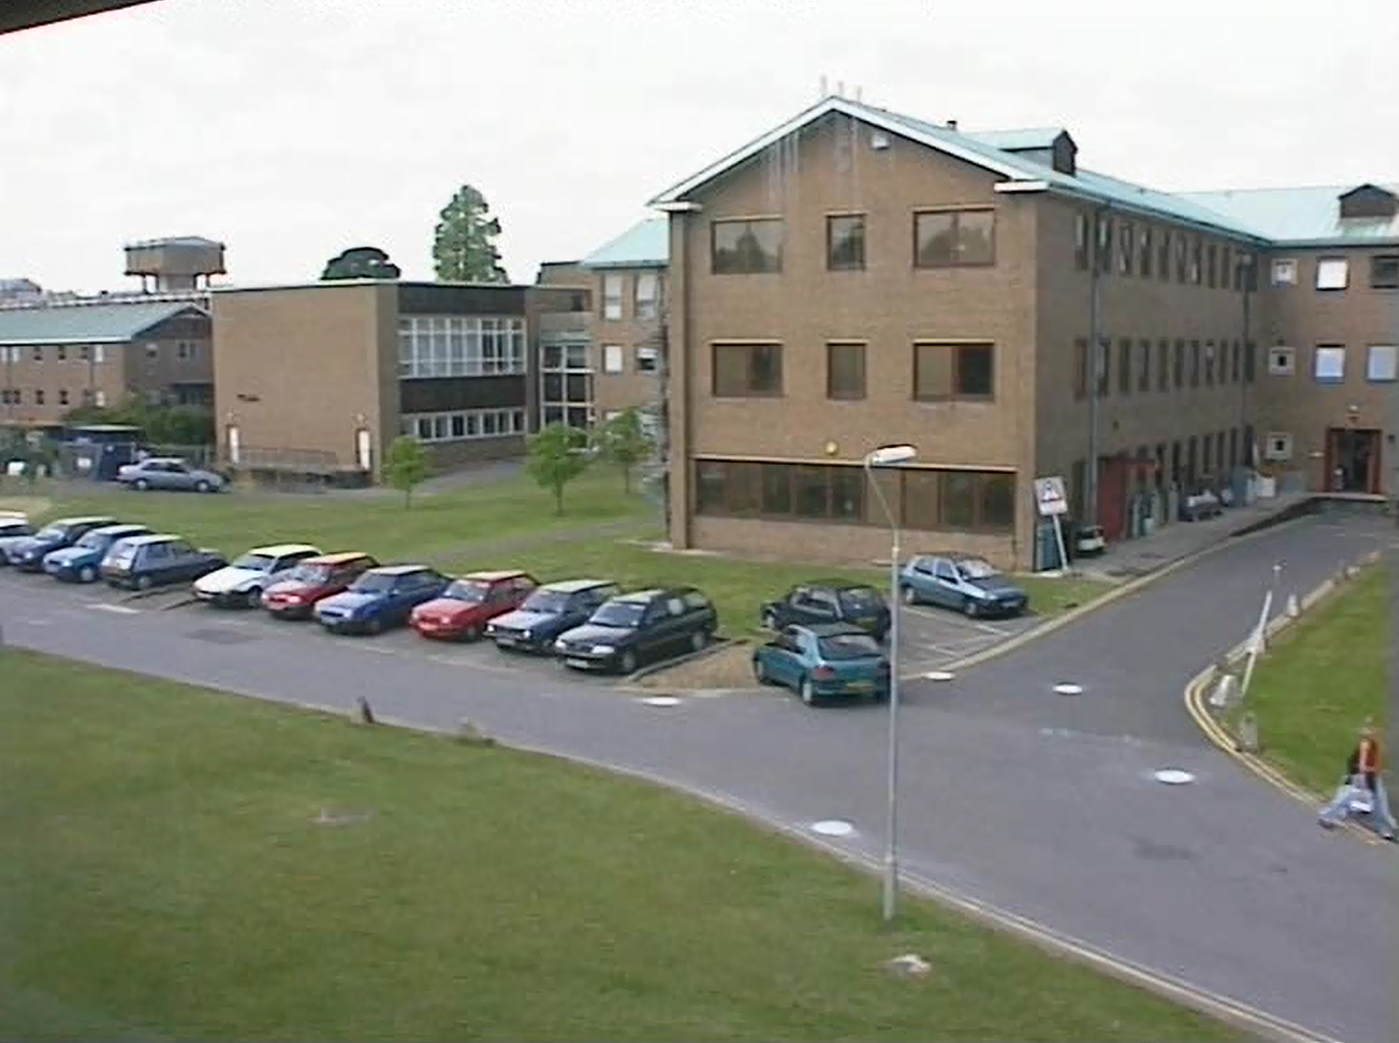
\includegraphics[width=\textwidth]{camReal}
%                 \caption{Test frame}
%                % \label{fig:gull}
%         \end{subfigure}%
%         ~ %add desired spacing between images, e. g. ~, \quad, \qquad etc.
%           %(or a blank line to force the subfigure onto a new line)
%         \begin{subfigure}[b]{0.5\textwidth}
%                 \centering
%                 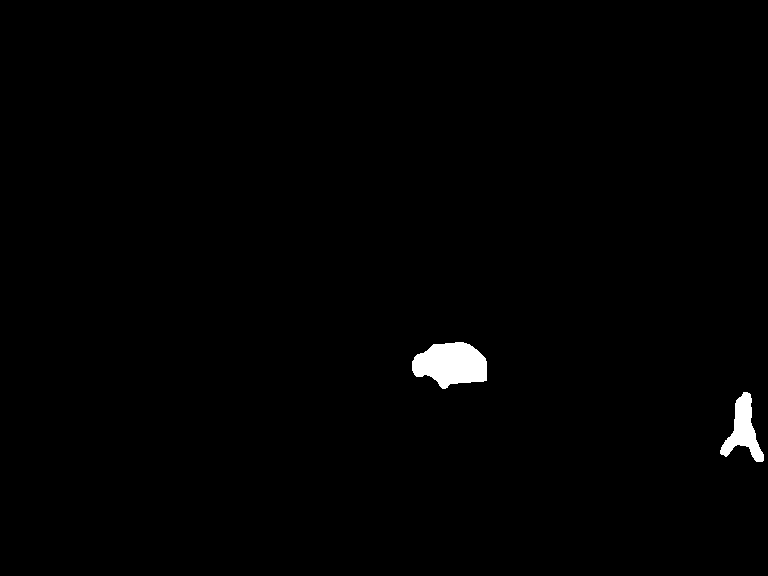
\includegraphics[width=\textwidth]{camGT}
%                 \caption{Ground truth}
%               %  \label{fig:tiger}
%         \end{subfigure}
% \caption{The spatial sparsity of foreground. A frame from the PETS data set  \cite{pets2001} and the corresponding foreground in white. }\label{fig:sparse}
% \end{figure}

% An early version of compressed sensing specifically for background subtraction was proposed in \cite{Cevher2008b}, and it is that framework which is followed in this report. 

% For each time step $t \in [1, \ldots, T]$ every frame $\boldsymbol{x_t}$ is modelled as the summation for the foreground and background as shown in equation \eqref{eq:6}.
% %
% \begin{equation}
%   \label{eq:6}
%   \boldsymbol{x}_t = \boldsymbol{f}_t + \boldsymbol{x^b}_t.
% \end{equation}
% %
% Each frame $\boldsymbol{x_t}$ is sensed with a measurement matrix $\boldsymbol{\Phi}$ using a method as discussed in Section \ref{sec:sensing-matrices}, which is then used to encode the frame as given in equation \eqref{eq:7}.

% \begin{equation}
%   \label{eq:7}
%  \boldsymbol{y}_t = \boldsymbol{\Phi} \boldsymbol{x}_t \; \forall t \in [1, \ldots, T]. 
% \end{equation}
% %
% Next a recovery procedure is chosen as discussed in Section \ref{sec:recovery-algorithms} which is represented by $\Delta(\boldsymbol{\Phi}, y)$. Cevher \cite{Cevher2008b} shows that in order to estimate the foreground we need to apply the recovery algorithm to the difference between the measurement vector  $\boldsymbol{y}_t$ and the estimated background $\boldsymbol{y}_t^b$, as in equation \eqref{eq:8}. This background is assumed to be known from an update procedure.  
% %
% \begin{equation}
%   \label{eq:8}
%  \boldsymbol{ \hat{f}}_t = \Delta(\boldsymbol{\Phi}, \boldsymbol{y}_t - \boldsymbol{y}_t^b).
% \end{equation}
% %
% equation \eqref{eq:8}, shows that the estimated foreground mask of the current frame $\boldsymbol{\hat{f_t}}$ can be found by applying a recovery algorithm on only compressed components, the information stored in lower dimension $\mathbb{R}^M$. Note that no knowledge of the original data $\boldsymbol{x}$ in full dimensional form $\mathbb{R}^N$ is required. It is this key fact that allows computational savings when applied on real video.  


% Throughout this procedure $\boldsymbol{\Phi}$ is selected beforehand, and this is kept fixed throughout. This means that no matter which frame is being analysed, the number of measurements taken $M$ will remain constant. This is not always ideal as the sparsity of images will not remain constant throughout a video. If too few compressive measurements are calculated, the foreground estimation may not fully capture the true foreground, resulting in an unreliable foreground mask. Whilst if too many measurements are taken, the extra measurements will not improve the quality of the foreground estimation but we will have wasted measurements, making the algorithm inefficient. \cite{Warnell2011} proposed a modification to this algorithm which has a static background but the number of measurements taken in each frame is adaptive. This method is known as adaptive rate compressive sensing (ARCS). 


% %Our method takes a vectorised form of the current frame $\boldsymbol{x_t}$, and acquires compressive measurements $\boldsymbol{y_t}$ of the frame using a Gaussian random matrix $\boldsymbol{\Phi}$. The foreground mask is then reconstructed by applying a recovery algorithm  to $(\boldsymbol{y_t} - \boldsymbol{y_t^b})$, where $\boldsymbol{y_b^t}$ is a compressed model for the background at time $t$. The silhouette is then thresholded to set any small values to zero, and the non-zero pixels are classified as foreground. 

% \subsection{Background Modelling}
% \label{sec:background-modelling}

% In order for this method to work well, it is important that a good model of the background is kept updated. Although a static background could be used for short indoor sequences, most real-world video sequences require a dynamic background model. \cite{piccardi2004background} suggests that a background model should be able to adapt to deal with illumination changes, high frequency repetitive background objects and changes in background geometry. 

% Illumination changes can be separated into gradual changes, or rapid changes. Gradual changes in illumination are mainly due to the light changing throughout the day. Rapid changes in illumination may occur when clouds cover the sun in outdoor scenes or a light being switched on or off in interior scenes.

% High frequency background objects are mainly found in outdoor footage such as leaves waving in the wind, water rippling or rainy weather. These small movements are actually part of the background so care should be taken to use an algorithm which detects them as such. Examples may also occur indoors but these are often less prominent. 

% Changes in background geometry refers to when part of the background begins to move. Examples of this are very common in real videos, such as a chair being repositioned in a room such as in \cite{Toyama1999} or a car driving into a car park as foreground, and then parking therefore becoming part of the background.

% In this report the background is modelled using a running average method as discussed in \cite{piccardi2004background} and \cite{Cossalter2009}. 
% This is calculated as in equation \eqref{eq:111}.
% \begin{equation}
%   \label{eq:111}
%   \boldsymbol{y_t^b} = \alpha \boldsymbol{y_t} + (1 - \alpha) \boldsymbol{y^b_{t-1}}
% \end{equation}
%  where $\alpha$ is a learning parameter.

% The initial background $\boldsymbol{y^b_0}$ is calculated by taking an average of scenes from a training set. If this information is not available it is possible to use only the first frame in the data set, but this may not be as accurate. The background model learning parameter $\alpha$ is tuned so that it is sensitive to the challenges discussed above, specifically to avoid the change in geometry problems. This challenge is especially prominent in the experimentation in Chapter \ref{cha:experiments} as the video used is CCTV footage is from a car park.   

% Now that the theory of compressive sensing with background subtraction has been introduced, the aim is to apply the recovery algorithms outlined in Section \ref{sec:recovery-algorithms} and evaluate their performance on a standard test video. 


%---------------- COMMENT FOR IMPORTING ----------------------
%\pagebreak											%Comment for importing
%\bibliographystyle{plainnat}		%Comment for importing
%\bibliography{References}				%Comment for importing
%\end{document}									%Comment for importing
%-------------------------------------------------------------
